\documentclass{article}
\usepackage{tikz}
\usepackage{amssymb}
\usepackage{amsthm}
\usepackage{amsmath}
\usepackage{mathabx}
\usepackage{listings}
\usepackage{bbm}
\usepackage{caption}
\usepackage{natbib}
\usepackage{float}
\usepackage{hyperref}
\usepackage{setspace}
\usepackage[margin = 1 in]{geometry}
\usepackage{tcolorbox}
\usetikzlibrary{patterns,automata,positioning,arrows}
\title{Strategy Free Machine Learning}
\author{-}
\date{\today}
\hbadness=99999

\begin{document}
\newtheorem{thm}{Theorem}
\newtheorem{cor}{Corollary}
\newtheorem{lem}{Lemma}
\newtheorem{prop}{Proposition}
\newtheorem{conj}{Conjecture}
\newtheorem{algo}{Algorithm}
\newtheorem{obs}{Observation}
\newtheorem{clm}{Claim}
\theoremstyle{definition}
\newtheorem{df}{Definition}
\newtheorem{eg}{Example}
\newtheorem{asm}{Assumption}
\newtheorem{cond}{Condition}
\theoremstyle{remark}
\newtheorem{rmk}{Remark}
\maketitle \onehalfspacing \allowdisplaybreaks \raggedbottom


\section{Short Summary} 
There are $n $ strategic agents each providing the label of one data point to the principal. The principal is the learner and builds a machine learning model based on the data points provided by the agents. An agent, $i $, has publicly known feature vector, $x_{i}$, and a private discrete label, $y_{i}$. The objective of the agent is to maximize the probability that her data point is labeled correctly by the principal's model, and the agent can choose to report $y^{\dagger}_{i}$ to achieve the objective, with the possibility of misreporting $y^{\dagger}_{i} \neq  y_{i}$. We say a dataset is incentive incompatible with respect to the learner, described by a parametric model, if at least one of the $n $ agents has the incentive to misreport.
\newline \newline
The following is the diagram showing a dataset that is incentive incompatible with respect to the multi-class logistic regression model. In the dataset, each of the $n  = 18$ agents, $i $, has a two dimensional feature vector and a private label can take on one of three values: "red", "green", or "blue".
\newline \newline
\begin{figure}[H] \centering 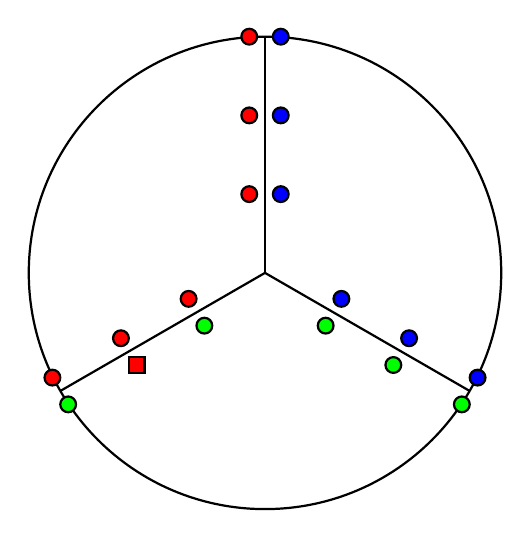
\begin{tikzpicture} [scale = 1] 
\draw[thick] (0.0, 0.0) circle [radius = 3.0];
\draw[thick] (0.0, 0.0) -- (0.0, 3.0);
\draw[fill = blue, thick] (0.2, 1.0) circle [radius = 0.1];
\draw[fill = blue, thick] (0.2, 2.0) circle [radius = 0.1];
\draw[fill = blue, thick] (0.2, 3.0) circle [radius = 0.1];
\draw[fill = red, thick] (-0.2, 1.0) circle [radius = 0.1];
\draw[fill = red, thick] (-0.2, 2.0) circle [radius = 0.1];
\draw[fill = red, thick] (-0.2, 3.0) circle [radius = 0.1];
\draw[thick] (0.0, 0.0) -- (2.6, -1.5);
\draw[fill = blue, thick] (0.97, -0.33) circle [radius = 0.1];
\draw[fill = blue, thick] (1.83, -0.83) circle [radius = 0.1];
\draw[fill = blue, thick] (2.7, -1.33) circle [radius = 0.1];
\draw[fill = green, thick] (0.77, -0.67) circle [radius = 0.1];
\draw[fill = green, thick] (1.63, -1.17) circle [radius = 0.1];
\draw[fill = green, thick] (2.5, -1.67) circle [radius = 0.1];
\draw[thick] (0.0, 0.0) -- (-2.6, -1.5);
\draw[fill = red, thick] (-0.97, -0.33) circle [radius = 0.1];
\draw[fill = red, thick] (-1.83, -0.83) circle [radius = 0.1];
\draw[fill = red, thick] (-2.7, -1.33) circle [radius = 0.1];
\draw[fill = green, thick] (-0.77, -0.67) circle [radius = 0.1];
\draw[fill = red, thick] (-1.73, -1.27) rectangle (-1.53, -1.07);
\draw[fill = green, thick] (-2.5, -1.67) circle [radius = 0.1];
\end{tikzpicture} \captionof{figure}{Incentive Incompatible Example}\label{fig:ic}
\end{figure}
The $18$ points are located inside a unit circle, and each point is $0.004$ away from the three line segments through the origin that form angles of $120$ degrees between them. There is one point, labeled by a square in the plot, that is on the "incorrect" side of the boundary. Suppose the point corresponds to the feature vector of an agent $i $ with private label "red", then truthfully reporting her label will lead to a multi-class logistic regression model that classifies her point as "green". The probability that this model classifies her point as "red" is $0.3290$. However, if the agent misreports her label as "blue", the resulting model classifies her point as "red" with probability $0.4966$. Therefore, by lying about her label, the agent is able to make the principal learn an incorrect model that classifies her point correctly and with a higher probability.
\newline \newline
The same dataset is also incentive incompatible with respect to the one-vs-rest linear support vector machine if the margin is used as the class "probabilities". However, in this case, the agent, with feature vector corresponding to the blue point close to the center and close to the green point, can only improve the margin slightly without making the model switch from classifying her point incorrectly to classifying her point correctly.
\newline \newline
However, this dataset is incentive compatible with respect to the Naive Bayes classifiers, and in general, there does not exist any dataset that is incentive incompatible with respect to discrete-valued Naive Bayes classifiers. Misreporting will always lead to lower posterior probability of the agent's true label. In addition, no dataset is incentive incompatible with respect to classifiers that minimizes empirical risk with zero-one loss.
\newline \newline



\section{Literature Review} 
Previous work on mechanism design for machine learning with strategic data sources focus on designing robust algorithms to incentivize the data providers to report their private data truthfully. Their models mainly differ in the objective and the possible actions of the data providers (agents) and the machine learner (principal).
\begin{itemize}
\item The first group of papers focuses on principal-agent problems in which each agent's private data point is the agent's type that the agent cannot change. The only action the agents can take is whether to report their private information truthfully.
\end{itemize}
\begin{enumerate}
\item Some models assume the agents' feature vectors are public, but their labels are private. \citet*{perote2004strategy}, \citet*{chen2018strategyproof}, and \citet*{gast2013linear} focus on strategy-proof linear regression algorithms and introduced clockwise repeated median estimators, generalized resistant hyperplane estimators, and modified generalized linear squares estimators. \citet*{dekel2010incentive} investigates the general regression problem with empirical risk minimization and absolute value loss. All the previously mentioned papers assume the labels are continuous variables (regression problems), and \citet*{meir2012algorithms} assumes the labels are discrete variables (classification problems) and proposes a class of random dictator mechanisms.
\item Some models assume the agents' feature vectors are also private. \citet*{chen2019grinding} investigates such problems for linear regressions.
\item Other models do not distinguish between feature vectors and labels. Each agent has a private valuation. These problems are usually modeled as facility locations problems and the solution involves some variant of the Vickrey-Clarke-Groves or Meyerson auction. These include \citet*{dutting2017optimal}, \citet*{golowich2018deep}, \citet*{epasto2018incentive}, and \citet*{procaccia2009approximate}.
\end{enumerate}

\begin{itemize}
\item The second group papers focus on moral-hazard problems in which each agent does not have a type but they can choose an action (with a cost) that affects the probability of obtaining the correct label. \citet*{richardsonprivately} focuses on the linear regression problem in this scenario, and \citet*{cai2015optimum} and \citet*{shah2016double} investigates the problem for more general machine learning problems. \citet*{mihailescu2010strategy} also discusses a similar problem for general machine learning algorithms.
\item The last group of papers uses machine learning or robust statistics techniques without game-theoretic models. This group of papers include \citet*{dekel2009vox}, \citet*{dekel2009good}.
\end{itemize}



\section{Logistic Regression} 

\subsection{Model and Example}
In this section, we assume the principal is training a multi-class logistic (softmax) regression. There are $n $ strategic agents each providing the label of one data point to the principal. An agent, $i $, with public feature vector, $x_{i} \in \mathbb{R}^{m}$, and private discrete label, $y_{i} \in \left\{1, 2, ..., k \right\}$, has the objective of maximizing the probability that her data point is labeled correctly by the principal's model, parameterized by the $m  \times \left(k  + 1\right)$ weights (and bias) matrix $w $. The agent can choose to report $y^{\dagger}_{i}$ to achieve the objective, with possibly $y^{\dagger}_{i} \neq  y_{i}$. Denoting the weights of the model resulting from the false report from agent $i $ by $w^\star \left(y^{\dagger}_{i}\right)$, the agent's objective can be written as,
\begin{align*}
&  \displaystyle\max_{y^{\dagger} \in \left\{1, 2, ..., k \right\}} \mathbb{P}\left\{Y = y_{i} | w^\star \left(y^{\dagger}_{i}\right), x_{i}\right\},
\end{align*}
where,
\begin{align*}
&  \mathbb{P}\left\{Y = c | w, x_{i}\right\} = \dfrac{e^{z_{i,c}}}{\displaystyle\sum_{c'=1}^{k} e^{z_{i,c'}}},
\\ &  z_{i,c} = \displaystyle\sum_{j=1}^{m} w_{j,c} x_{i,j} + b_{c} , \text{\;for\;} c \in \left\{1, 2, ..., k\right\}.
\end{align*}
The principal is not strategic and he maximizes the likelihood of the data,
\begin{align*}
&\displaystyle\max_{w} \displaystyle\sum_{i=1}^{n} \log\left(\mathbb{P}\left\{Y = y^{\dagger}_{i} | w, x_{i}\right\}\right).
\end{align*}
We consider the case without coalition of group of agents, so only one agent is misreporting at a time, and use the following notations,
\begin{align*}
w^\star  &= \arg\displaystyle\max_{w} \displaystyle\sum_{i=1}^{n} \log\left(\mathbb{P}\left\{Y = y_{i} | w, x_{i}\right\}\right)
\\ w^\star \left(y^{\dagger}_{i}\right) &= \arg\displaystyle\max_{w} \log\left(\mathbb{P}\left\{Y = y^{\dagger}_{i} | w, x_{i}\right) + \displaystyle\sum_{i' = 0, i' \neq  i}^{n} \log\left(\mathbb{P}\left\{Y = y_{i'} | w, x_{i'}\right\}\right),\right.
\end{align*}
\begin{df} \label{df:ic} 
A dataset is incentive incompatible with respect to a learner if there exists at least one agent $i $, and some $y^{\dagger}_{i} \neq  y_{i}$ such that,
\begin{align*}
\mathbb{P}\left\{Y = y_{i} | w^\star , x_{i}\right\} &< \mathbb{P}\left\{Y = y_{i} | w^\star \left(y^{\dagger}_{i}\right), x_{i}\right\}.
\end{align*}
A learner (algorithm) is incentive compatible if there does not exist a dataset that is incentive incompatible.
\newline \newline\end{df}
\begin{prop} \label{prop:logit} 
Multi-class logistic regression is not incentive compatible.
\end{prop}
\begin{proof} \label{proof:logitpf} 
The example given previously is a dataset that is incentive incompatible.
\newline \newline\end{proof}
\begin{figure}[H] \centering 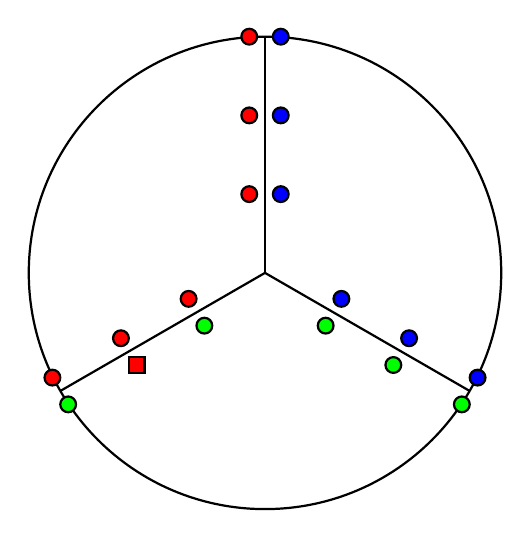
\begin{tikzpicture} [scale = 1] 
\draw[thick] (0.0, 0.0) circle [radius = 3.0];
\draw[thick] (0.0, 0.0) -- (0.0, 3.0);
\draw[fill = blue, thick] (0.2, 1.0) circle [radius = 0.1];
\draw[fill = blue, thick] (0.2, 2.0) circle [radius = 0.1];
\draw[fill = blue, thick] (0.2, 3.0) circle [radius = 0.1];
\draw[fill = red, thick] (-0.2, 1.0) circle [radius = 0.1];
\draw[fill = red, thick] (-0.2, 2.0) circle [radius = 0.1];
\draw[fill = red, thick] (-0.2, 3.0) circle [radius = 0.1];
\draw[thick] (0.0, 0.0) -- (2.6, -1.5);
\draw[fill = blue, thick] (0.97, -0.33) circle [radius = 0.1];
\draw[fill = blue, thick] (1.83, -0.83) circle [radius = 0.1];
\draw[fill = blue, thick] (2.7, -1.33) circle [radius = 0.1];
\draw[fill = green, thick] (0.77, -0.67) circle [radius = 0.1];
\draw[fill = green, thick] (1.63, -1.17) circle [radius = 0.1];
\draw[fill = green, thick] (2.5, -1.67) circle [radius = 0.1];
\draw[thick] (0.0, 0.0) -- (-2.6, -1.5);
\draw[fill = red, thick] (-0.97, -0.33) circle [radius = 0.1];
\draw[fill = red, thick] (-1.83, -0.83) circle [radius = 0.1];
\draw[fill = red, thick] (-2.7, -1.33) circle [radius = 0.1];
\draw[fill = green, thick] (-0.77, -0.67) circle [radius = 0.1];
\draw[fill = red, thick] (-1.73, -1.27) rectangle (-1.53, -1.07);
\draw[fill = green, thick] (-2.5, -1.67) circle [radius = 0.1];
\end{tikzpicture} \captionof{figure}{Incentive Incompatible Example}\label{fig:icr}
\end{figure}
In this example, agent $i $ reports $x_{i} \in \mathbb{R}^{2}$ and $y_{i}$ is one of $1$ (red), $2$ (green), or $3$ (blue). Suppose the red square point correspond to agent $1$ with $x_{1} = \left(-1.63, -1.17\right)$ and $y_{1} = 1$.
\begin{align*}
\mathbb{P}\left\{Y = 1 | w^\star , x_{1}\right\} &= 0.3290,
\\ \mathbb{P}\left\{Y = 1 | w^\star \left(y^{\dagger}_{1} = 3\right), x_{1}\right\} &= 0.4966.
\end{align*}
Here, parameter estimation is done using maximum likelihood estimation with BFGS, and $w^\star $ is given by, with class $1$ weights normalized to $0$,
\begin{center} \begin{tabular}{|c|c|c|c|c|}
\hline
 Class &(Intercept) &x1 &x2\\ \hline
$2$ &-$0.6053178$ &$104.9925$ &-$181.3391914$\\ \hline
$3$ &-$0.2852057$ &$209.4190$ &$0.3656777$\\ \hline
\end{tabular} \end{center}
and $w^\star \left(y^{\dagger}_{1} = 3\right)$ is given by,
\begin{center} \begin{tabular}{|c|c|c|c|c|}
\hline
 Class &(Intercept) &x1 &x2\\ \hline
$2$ &-$0.1915645$ &$3.473426$ &-$5.507418$\\ \hline
$3$ &$0.8273350$ &$4.309293$ &-$1.200060$\\ \hline
\end{tabular} \end{center}


\subsection{Incentive Incompatibility}
To characterize the set of incentive incompetible datasets, we rewrite the principal's choice of optimal weights by,
\begin{align*}
w^\star  &= \arg\displaystyle\max_{w} \log\left(\mathbb{P}\left\{Y = y_{i} | w, x_{i}\right\}\right) + C_{-i}\left(w\right),
\end{align*}
where the function $C_{-i}\left(w\right)$ summarizes the loss due to agents other than $i $, assuming they are reporting labels truthfully,
\begin{align*}
C_{-i}\left(w\right) &= \displaystyle\sum_{i' = 0, i' \neq  i}^{n} \log\left(\mathbb{P}\left\{Y = y_{i'} | w, x_{i'}\right\}\right).
\end{align*}
Since the objective is globally convex and differentiable, as shown in , the problem translates to the first derivative condition,
\begin{align*}
\dfrac{\nabla _{w} \mathbb{P}\left\{Y = y_{i} | w^\star , x_{i}\right\}}{\mathbb{P}\left\{Y = y_{i} | w^\star , x_{i}\right\}} + \nabla _{w} \left(C_{-i}\left(w^\star \right)\right) &= 0,
\\ \dfrac{\nabla _{w} \mathbb{P}\left\{Y = y^{\dagger}_{i} | w^\star \left(y^{\dagger}_{i}\right), x_{i}\right\}}{\mathbb{P}\left\{Y = y^{\dagger}_{i} | w^\star \left(y^{\dagger}_{i}\right), x_{i}\right\}} + \nabla _{w} \left(C_{-i}\left(w^\star \left(y^{\dagger}_{i}\right)\right)\right) &= 0.
\end{align*}
For logistic regression with weights $w_{c}, c = 1, 2, ..., k $, without normalization,
\begin{align*}
\mathbb{P}\left\{Y = c | w, x\right\} &= \dfrac{e^{w_{c}^{T} x + b_{c}}}{\displaystyle\sum_{c'} e^{w_{c'}^{T} x + b_{c'}}},
\\ \nabla _{w_{c}} \mathbb{P}\left\{Y = c | w, x\right\} &= \dfrac{e^{w_{c}^{T} x + b_{c}} \displaystyle\sum_{c' \neq  c} e^{w_{c}^{T} x + b_{c}}}{\left(\displaystyle\sum_{c'} e^{w_{c'}^{T} x + b_{c'}}\right)^{2}} x.
\\ \nabla _{w_{c}} \mathbb{P}\left\{Y = \hat{c}, \hat{c} \neq  c | w, x\right\} &= \dfrac{e^{w_{c}^{T} x + b_{c}} e^{w_{\hat{c}}^{T} x + b_{\hat{c}}}}{\left(\displaystyle\sum_{c'} e^{w_{c'}^{T} x + b_{c'}}\right)^{2}} x.
\end{align*}
The derivative conditions implies,
\begin{align*}
\left(1 - \mathbb{P}\left\{Y = c | w^\star , x_{i}\right\}\right) x_{i} + \nabla _{w_{c}} \left(C_{-i}\left(w^\star \right)\right) &= 0, c = y_{i,}
\\ \left(\mathbb{P}\left\{Y = c | w^\star , x_{i}\right\}\right) x_{i} + \nabla _{w_{c}} \left(C_{-i}\left(w^\star \right)\right) &= 0, c \neq  y_{i,}
\end{align*}
same for the expression with $w^\star \left(y^{\dagger}_{i}\right)$.
\\* Substitute into the incentive incompatibility condition,
\begin{align*}
\nabla _{w_{y_{i} ,j}} \left(C_{-i}\left(w^\star \right)\right)) x_{i,j} &\leq  \nabla _{w_{y_{i} ,j}} \left(C_{-i}\left(w^\star \left(y^{\dagger}_{i}\right)\right)\right) x_{i,j}, j = 1, 2, ..., m. 
\end{align*}


\subsection{Continuous Label}
The previous formulation does not permit $y^{\dagger}_{i}$ to be a continous variable, but if we rewrite the optimization as the maximization of the cross entropy, then we could treat $y^{\dagger}_{i} \in \Delta^{K-1}$ as a continous multinomial distribution where $y^{\dagger}_{i,c} \in \left[0, 1\right]$ denotes the probability of agent $i $ reporting label $c \in \left\{1, 2, ..., K\right\}$. The principal's problem can be rewritten as,
\begin{align*}
&\displaystyle\min_{w} \displaystyle\sum_{i=1}^{n} \displaystyle\sum_{c=1}^{K} -y^{\dagger}_{i,c} \log\left(\mathbb{P}\left\{Y = c | w, x_{i}\right\}\right).
\end{align*}
Assuming $w^\star \left(y^{\dagger}_{i}\right)$ is the optimal weights, the objective function becomes,
\begin{align*}
\mathcal{L}\left(w, y^{\dagger}_{i}\right) &= \displaystyle\sum_{c=1}^{k} \hat{-y}_{i,c} \log\left(\mathbb{P}\left\{Y = c | w, x_{i}\right\}\right) - \displaystyle\sum_{i' =1, i' \neq  i}^{n} \log\left(\mathbb{P}\left\{Y = y_{i'} | w, x_{i'}\right\}\right),
\end{align*}
and the value function is,
\begin{align*}
\mathcal{L}^\star \left(y^{\dagger}_{i}\right) &= \displaystyle\sum_{c=1}^{k} \hat{-y}_{i,c} \log\left(\mathbb{P}\left\{Y = c | w^\star \left(y^{\dagger}_{i}\right), x_{i}\right\}\right) - \displaystyle\sum_{i' =1, i' \neq  i}^{n} \log\left(\mathbb{P}\left\{Y = y_{i'} | w^\star \left(y^{\dagger}_{i}\right), x_{i'}\right\}\right),
\end{align*}
and apply the envolope theorem,
\begin{align*}
\dfrac{\partial \mathcal{L}^\star \left(y^{\dagger}_{i}\right)}{\partial y^{\dagger}_{i}} &= -\log\left(\mathbb{P}\left\{Y = y^{\dagger}_{i} | w^\star \left(y^{\dagger}_{i}\right), x_{i}\right\}\right)
\\ &> 0.
\end{align*}
Alternatively, if gradient descent is used in the optimization process, one iteration of the gradient descent with learning rate $\eta$ is given by,
\begin{align*}
w'_{j,c} &= w_{j,c} - \eta x_{i,j} \left(\mathbb{P}\left\{Y = c | x_{i}\right\} - \mathbbm{1}_{y^{\dagger}_{i}}\right).
\end{align*}
Now fix instance $i $ and define $o_{c} = \mathbb{P}\left\{Y = c | x_{i}\right\}$, then,
\begin{align*}
\dfrac{\partial o_{c}}{\partial y_{c}} &= \dfrac{\partial o_{c}}{\partial z_{c}} \displaystyle\sum_{j=1}^{m} \dfrac{\partial z_{c}}{\partial w_{j,c}} \dfrac{\partial w_{j,c}}{\partial y_{c}}
\\ &= o_{c} \left(1 - o_{c}\right) \displaystyle\sum_{j=1}^{m} x_{j}^{\left(i\right)} x_{j}^{\left(i\right)} \eta
\\ &= \eta o_{c} \left(1 - o_{c}\right) \displaystyle\sum_{j=1}^{m} \left(x_{j}^{\left(i\right)}\right)^{2}
\\ &\geq  0.
\end{align*}
Similarly,
\begin{align*}
\dfrac{\partial o_{c}}{\partial y_{c'}} &= \dfrac{\partial o_{c}}{\partial z_{c'}} \displaystyle\sum_{j=1}^{m} \dfrac{\partial z_{c'}}{\partial w_{j,c'}} \dfrac{\partial w_{j,c'}}{\partial y_{c'}}
\\ &= - o_{c} o_{c'} \displaystyle\sum_{j=1}^{m} x_{j}^{\left(i\right)} x_{j}^{\left(i\right)} \eta
\\ &= - \eta o_{c} o_{c'} \displaystyle\sum_{j=1}^{m} \left(x_{j}^{\left(i\right)}\right)^{2}
\\ &\leq  0.
\end{align*}
This implies decreasing $y_{i,c}$ and thus increasing $y_{i,c'}$ for some $c'$ will always increase $o_{c}$. Therefore, there should be no incentive to misreport by changing $y^{\dagger}_{i}$ slightly from $y_{i.}$
\newline \newline


\subsection{Zero-One Loss Logistic Regression}
With zero-one loss, in general, for an agent with label $y, $
\\* If $\hat{y} = y $, misreporting could only make $\hat{y} \neq  y$.
\\* If $\hat{y} \neq  y, $
\begin{enumerate}
\item switching to report $\hat{y}$ would improve the zero-one loss, and will not change the prediction $\hat{y}$. It is impossible to increase the loss by more than $1$, because if it were possible, then the original model was not optimal.
\item switching to $y' \neq  \hat{y}$ would keep the same zero-one loss, and will either not change the prediction $\hat{y}$, or will change the prediction to $y' \neq  y $, which does not make the agent better off.
\end{enumerate}





\section{Naive Bayes Model} 
No example in which agents have incentive to misreport is found for the Gaussian Naive Bayes estimator.
\newline \newline
The prediction is given by:
\begin{align*}
&\arg\displaystyle\max_{c} \mathbb{P} \left\{Y = c\right\} \mathbb{P} \left\{x^{\left(i\right)} | Y = c\right\}
\end{align*}
Consider agent $i $ with $\left(x^{\left(i\right)}, y^{\left(i\right)}\right)$, if she reports truthfully,
\begin{align*}
\mathbb{P} \left\{Y = y^{\left(i\right)}\right\} &= \left(\dfrac{n_{y^{\left(i\right)}}}{n},\right.
\\ \mathbb{P} \left\{x^{\left(i\right)} | Y = y^{\left(i\right)}\right\} &\geq  \mathbb{P} \left\{x^{\left(i\right)} | Y = \hat{y}\right\},
\end{align*}
and if she reports $\hat{y} \neq  y^{\left(i\right)}$,
\begin{align*}
\mathbb{P} \left\{Y = y^{\left(i\right)}\right\} &= \dfrac{n_{y^{\left(i\right)}} - 1}{n},
\\ \mathbb{P} \left\{x^{\left(i\right)} | Y = y^{\left(i\right)}\right\} &\leq  \mathbb{P} \left\{x^{\left(i\right)} | Y = \hat{y}\right\},
\end{align*}
and both terms are smaller.
\newline \newline
Given the dataset, the parameters $w  = \left(\mu, \Sigma, \pi\right)$ (mean, variance, prior) are given by,
\begin{align*}
\mu_{c} &= \dfrac{\displaystyle\sum_{i'=1}^{n} x^{\left(i'\right)} \mathbbm{1}_{y^{\left(i'\right)} = c}}{n_{c}},
\\ \Sigma_{c} &= \dfrac{\displaystyle\sum_{i'=1}^{n} \left(x^{\left(i'\right)} - \mu_{c}\right) \left(x^{\left(i'\right)} - \mu_{c}\right)^{T} \mathbbm{1}_{y^{\left(i'\right)} = c}}{n_{c}},
\\ \pi_{c} &= \dfrac{n_{c}}{n} .
\end{align*}
Then, the classification probability is,
\begin{align*}
\mathbb{P}_{c} \left\{Y = c | x^{\left(i\right)}\right\} &\propto \pi_{c} \dfrac{1}{\left| \Sigma_{c} \right|} \exp\left(- \dfrac{1}{2} \left(x^{\left(i\right)} - \mu_{c}\right)^{T} \left(\Sigma_{c}\right)^{-1} \left(x^{\left(i\right)} - \mu_{c}\right)\right).
\end{align*}
The condition for incentive compatibility is,
\begin{align*}
\pi'_{c} \dfrac{1}{\left| \Sigma'_{c} \right|} \exp\left(- \dfrac{1}{2} \left(x^{\left(i\right)} - \mu'_{c}\right)^{T} \left(\Sigma'_{c}\right)^{-1} \left(x^{\left(i\right)} - \mu'_{c}\right)\right) &< \pi_{c} \dfrac{1}{\left| \Sigma_{c} \right|} \exp\left(- \dfrac{1}{2} \left(x^{\left(i\right)} - \mu_{c}\right)^{T} \left(\Sigma_{c}\right)^{-1} \left(x^{\left(i\right)} - \mu_{c}\right)\right),
\end{align*}
where,
\begin{align*}
\mu'_{c} &= \dfrac{\displaystyle\sum_{i' \neq  i} x^{\left(i'\right)} \mathbbm{1}_{y^{\left(i'\right)} = c}}{n_{c} - 1},
\\ \Sigma'_{c} &= \dfrac{\displaystyle\sum_{i' \neq  i} \left(x^{\left(i'\right)} - \mu_{c}\right) \left(x^{\left(i'\right)} - \mu_{c}\right)^{T} \mathbbm{1}_{y^{\left(i'\right)} = c}}{n_{c} - 1},
\\ \pi'_{c} &= \dfrac{n_{c} - 1}{n} .
\end{align*}
In one-dimensional case, if agent $i $ with $x^{\left(i\right)}$ and label $y^{\left(i\right)} = c $ reports truthfully,
\begin{align*}
\mathbb{P} \left\{Y = c | x^{\left(i\right)}\right\} &= \dfrac{1}{\sigma_{c} \sqrt{2 \pi}} \exp\left(- \dfrac{\left(x^{\left(i\right)} - \mu_{c}\right)^{2}}{2 \sigma_{c}^{2}}\right),
\\ \mathbb{P}' \left\{Y = c | x^{\left(i\right)}\right\} &= \dfrac{1}{\sigma'_{c} \sqrt{2 \pi}} \exp\left(- \dfrac{\left(x^{\left(i\right)} - \mu'_{c}\right)^{2}}{2 \left(\sigma'_{c}\right)^{2}}\right),
\end{align*}
where,
\begin{align*}
\mu'_{c} &= \dfrac{n_{c} \mu}{n_{c} - 1} - \dfrac{x^{\left(i\right)}}{n_{c} - 1} ,
\\ \left(\sigma'_{c}\right)^{2} &= \dfrac{n_{c} \sigma_{c}^{2}}{n_{c} - 1} - \dfrac{\left(x^{\left(i\right)} - \mu_{c}\right) \left(x^{\left(i\right)} - \mu'_{c}\right)}{n_{c} - 1}
\\ &= \dfrac{n_{c} \sigma_{c}^{2}}{n_{c} - 1} - \dfrac{n_{c} \left(x^{\left(i\right)} - \mu_{c}\right)^{2}}{\left(n_{c} - 1\right)^{2}} .
\end{align*}
If $x^{\left(i\right)} > \mu_{c}$, then $\mu'_{c} < \mu_{c}$, but it is not clear how $\sigma'_{c}$ and $\sigma_{c}$ compares? Is it possible to have the following scenario?
\begin{figure}[H]
\centering
\includegraphics[width=0.5\linewidth]{normal}
\caption{Normal Means}
\end{figure}
 -
\newline \newline



\section{Support Vector Machines} 

\subsection{One-vs-One}
Since binary SVM is incentive compatible, no agent can gain from misreporting in any of the one-vs-one SVMs. Therefore, there will be no incentive to misreport in the multi-class SVM.
\newline \newline


\subsection{One-vs-Rest}
If margin is used as the prediction probabilities, then it is possible to improve the margin by misreporting the third class label, for example on the $18$-point data set.
\newline \newline


\subsection{Tree-Based}
Since binary SVM is incentive compatible, no agent can gain from misreporting in any stage. Therefore, there will be no incentive to misreport in the multi-class SVM.
\newline \newline




\section{Numerical Results} 

\subsection{Structured Examples}
A dataset is incentive incompatible with respect to the model parameterized by $w $ if at least one agent has the incentive to report $\hat{y} ^{\left(i\right)} \neq  y^{\left(i\right)}$. Formally, let the model estimated with the true label be,
\begin{align*}
w^\star  &= \arg\displaystyle\max_{w} \displaystyle\sum_{i'=1^{n}} \log\left(\mathbb{P}\left\{Y = y^{\left(i'\right)} | w, x^{\left(i'\right)}\right\}\right) + \lambda \left\|w\right\|,
\end{align*}
and the model estimated with the misreported label be,
\begin{align*}
\hat{w} &= \arg\displaystyle\max_{w} \left(\displaystyle\sum_{i' \neq  i} \log\left(\mathbb{P}\left\{Y = y^{\left(i'\right)} | w, x^{\left(i'\right)}\right\}\right)\right) + \log\left(\mathbb{P}\left\{Y = \hat{y} ^{\left(i\right)} | w, x^{\left(i\right)}\right\}\right) + \lambda \left\|w\right\|.
\end{align*}
The parameter $\lambda$ is the regulerization parameter.
\\* The dataset is incentive incompatible if there is $i $ such that,
\begin{align*}
\mathbb{P}\left\{Y = y^{\left(i\right)} | \hat{w}, x^{\left(i\right)}\right\} &> \mathbb{P}\left\{Y = y^{\left(i\right)} | w^\star , x^{\left(i\right)}\right\}.
\end{align*}
\bibliographystyle{te}
\bibliography{cs}


\end{document}
